% \documentclass{article}
% \usepackage{xeCJK}
% \usepackage{tikz}
% \usetikzlibrary{decorations.pathreplacing, calligraphy}
% \usetikzlibrary{quotes,angles}
% \begin{document}
\begin{tikzpicture}
    \node at (0,0) {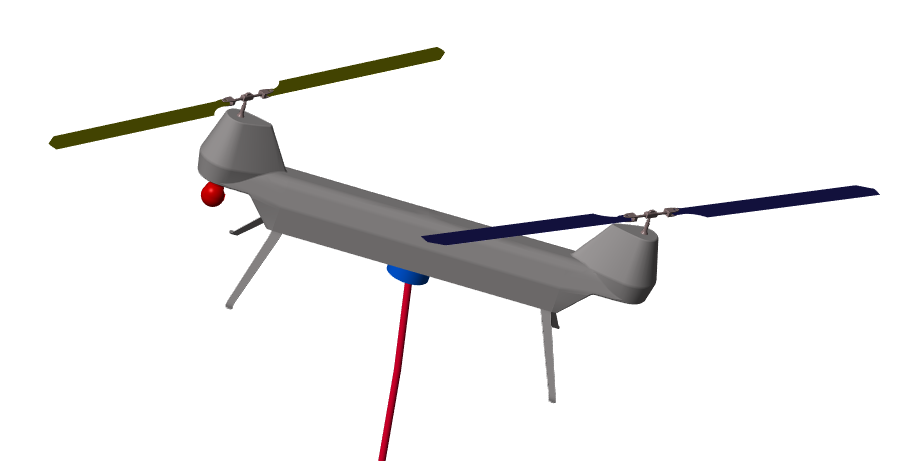
\includegraphics[width = 5cm]{tandem.PNG}};
    \draw[-latex] (-1,-2) -- (-2.5,-2) node[above] {飞行方向}; 
    \draw (-0.3,-0.1) node[right, yshift = -0.2cm]{$O_{b,1}^y$} node[right, yshift = -0.6cm]{$O_{b,1}$};
    % 绕y轴旋转
    \draw[-latex] (-0.3,-0.1) -- (-3.,0.7) node[above] {$X_{b,1}^y$};
    \draw[-latex] (-0.3,-0.1) -- (1.5,1.4) node[right] {$Y_{b,1}^y$}; 
    \draw[-latex] (-0.3,-0.1) -- (-0.65,-2) node[right,yshift = 0.4cm] {$Z_{b,1}^y$}; 
     % 绕x轴旋转
     \draw[-latex] (-0.3,-0.1) -- (-3.,0.7) node[below] {$X_{b,1}$};
     \draw[-latex] (-0.3,-0.1) -- (1.5,1.0) node[right] {$Y_{b,1}$}; 
     \draw[-latex] (-0.3,-0.1) -- (-0.95,-1.9) node[left,yshift = 0.4cm] {$Z_{b,1}$};   
     \draw
    (1.5,1.0) coordinate (a)
    (-0.3, -0.1) coordinate (b)
    (1.5,1.4) coordinate (c)
    pic["$\phi_1$", draw=orange, <-, angle eccentricity=1.2, angle radius=1.5cm]
    {angle=a--b--c};
\end{tikzpicture}  

% \end{document}